\documentclass[12pt]{article}
\usepackage{fullpage,graphicx,psfrag,amsmath,amsfonts,verbatim}
\usepackage[small,bf]{caption}
\usepackage{amsthm}
\usepackage{hyperref}
\usepackage{bbm} % for the indicator function to look good
\usepackage{color}
\usepackage{mathtools}
\input newcommand.tex


% \bibliographystyle{alpha}

\title{Econometrics 2: Non-parametric methods }
\author{Eric Gautier\thanks{Notes by FU Zixuan, last compiled on \today.}}
\date{2024 Spring}

\begin{document}
\maketitle

\begin{figure*}[h]
    \centering
    
\includegraphics{figures/ihaveaquestion.jpg}
    \caption*{I have a question!}
\end{figure*}



\newpage
\tableofcontents
\newpage

\section{Preliminaries}
\subsection{Probability basics}
\begin{definition}[distribution law]
    The distribution law of a random variable $X$ is $\p_X$ is the probability on $\pa{\Rd,\calb\pa{\Rd}}$ such that  $\p_X\bra{B}=\p\bra{X\in B}$ for all $B\in \calb\pa{\Rd}$
\end{definition}

\begin{definition}[density]
    $X$ has density $f_X$ if $\p_X\bra{B}=\int_B \underbrace{f_X(x)dx}_{d\p_X(x)}$ for all $B\in \calb\pa{\Rd}$
\end{definition}

Let $Y$ be a random variable and $X$ be a random vector in $\Rd$ defined on the same probability space $\pspace$. We want to define and manipulate $\E\bra{Y|X}$.

There are 2 particular cases
\begin{enumerate}
    \item $\pa{Y,X^\top}^\top$ has discrete support. Let $x\in \text{spt}(X)$, then $\E\bra{Y|X=x}=\sum y_j \p\pa{Y=y_j\mid X=X}$. This is well defined only when $\p\pa{X=x}>0$ in which case $\p\pa{Y=y_j\mid X=x}=\frac{\p\pa{Y=y_j,X=x}}{\p\pa{X=x}}$ is well defined.
    \item $\pa{Y,X^\top}^\top$ and $X$ have a density then $\E\bra{Y|X=x}=\int yf_{Y|X=x}(y)dy$ where $f_{Y|X=x}(y)=\frac{f_{Y,X}(y,x)}{f_X(x)}$.
\end{enumerate}
\begin{proposition}[conditional expectation]
    The random variabel $Z \coloneqq \E\bra{Y|X}$ is the unique random variable such that
    \begin{enumerate}
        \item $Z\in L^1\pspace$, that is $Z$ is $\sigma(X)$-measurable.
        \item \label{prop:con_exp_uniqueness}$\E\bra{Z\mathbbm{1}_B}=\E\bra{Y\mathbbm{1}_B}$ for all $B\in \sigma(X)$.
    \end{enumerate}
    \emph{unique} means that if $Z'$ is another random variable satisfying the same properties, then $Z=Z'$ a.s.
\end{proposition}
\begin{remark}
    The random variable $Z$ is $\sigma(X)$-measurable iff $Z=\phi(X)$ for some function $\phi:\pa{\Rd,\calb\pa{\Rd}}\to\pa{\R,\calb\pa{\R}}$. The corresponding function $\phi$ for $Z=\underbrace{E\bra{Y|X}}_{\text{conditional expectation}}$ is denoted by $\underbrace{\E\bra{Y|X=x}}_\text{conditional expectation function}$.
\end{remark}
\begin{remark}
    The proposition \ref{prop:con_exp_uniqueness} is equivalent to 
    \begin{align*}
        &\E\bra{\pa{Y-Z}\mathbbm{1}_B}=0, \quad \forall B\in \sigma(X) \\ \Leftrightarrow &\E\bra{\pa{Y-Z}\psi(X)}=0, \quad \forall \psi\ \text{bounded and meansurable}.
    \end{align*}
\end{remark}

\begin{exercise}
    Let $X$ and $\beta$ be random vectors in $\Rd$ such that $X$ and $\beta$ ARE independent, that is $\p_{X,\beta}=\p_X \times \p_\beta$. Let $g:\Rd\to\R$ be a bounded and measurable function. Define $Y=g(X^\top\beta)$. It can be shown that $\E\bra{Y|X=x}=\E\bra{g(x^\top\beta)}$ for all $x\in \text{supp}(X)$.
\end{exercise}
\begin{proof}
    Let $B\in \sigma(X)$. Then $$\E\bra{Y\1\{X\in B\}}=\E\bra{g(X^\top\beta)\1\{X\in B\}}=\int\int g(X^\top b)\1{x\in B}d\p_{\beta,X}(b,x).$$ 
    Since $X$ and $\beta$ are independent, we have $$\p_{\beta,X}(b,x)=\p_X(x)\p_\beta(b).$$
    Therefore, \begin{equation*}
        \begin{split}
            \E\bra{Y\1\{X\in B\}}&=\int\int g(x^\top b)\1\{x\in B\}d\p_{\beta}(b)d\p_X(x) \\&=\int \E\bra{g(x^\top \beta)}\1\{x\in B\}d\p_X(x)\\
            &=\E\bra{\E\bra{g(x^\top \beta)}\1\{X\in B\}}\\
            &=\E\bra{\phi(X)\1\{X\in B\}}
        \end{split}
    \end{equation*}
    where $ \E\bra{g(x^\top \beta)}\equiv \phi(x)$ takes expectation over $\beta$ and is a function of $x$.
    By the uniqueness of conditional expectation, we have $\E\bra{Y|X}=\E\bra{\phi(X)}$.
\end{proof}

\subsection{Completeness condition}

We want to understand the completeness condition when $X=Z-\eta$, where $Z \indep \eta$ and both have densities. 
Recall the definition of \textbf{completeness}.
\begin{definition}[Completeness]
\label{completeness}
Completeness is defined as such that $$
\forall z \in \R,\ \int_\R \varphi(x)f_\eta(z-x)dx=0 \text{ implies that for all } x,\ \varphi(x)=0,$$
where $\varphi$ is continuous and $\int_\R  \abs{{\varphi(x)}}dx <\infty$.
\end{definition}
Now, We make a detour to introduce some notations in function space.
\begin{definition}
    Let $f$ be a function defined on $\Rd$ with values in $\R$ or $\C$ and $p\le 1$. Then $L^p(\Rd)$ is defined as the space of measurable function from $\left(\Rd,\mathcal{B}(\Rd)\right)$ such that $\int_{\Rd}\abs{f(x)}^p dx<\infty$. If $f$ takes value from $\C$, $\abs{\cdot}$ is the modulus. 
\end{definition}

\begin{definition} [$L^1\pa{\R}$ space]
        A function is in $L^1\pa{\R}$ if $\int_{\R} \abs{f\pa{x}}dx <\infty$.
\end{definition}
\begin{definition}[Fourier transform]
	If $f\in L^1\pa{\R}$, the Fourier transform of $f$ is defined for all $w\in \R$ by
	\begin{equation*}
		\F\bra{f}\pa{w} = \int_\R e^{iwx} f\pa{x}dx.
	\end{equation*}
\end{definition}
\begin{remark}
    Let $t\in \R$, $e^{it}=\cos(t)+i\sin(t)$ and $\abs{e^{it}}^2=1$
\end{remark}
\begin{definition}[Convolution]
    If $f$ and $g$ belong to $L^1(\Rd)$, the convolution of $f$ and $g$ is $f\ast g(z)=\int f(x)g(z-x)dx$.
\end{definition}
\begin{proposition}
    If $f$ and $g$ belong to $L^1(\Rd)$, then $f\ast g \in L^1(\Rd)$. Its Fourier transformation is $F\bra{f\ast g}(w)=F\bra{f}(w)=F\bra{f}(w)F\bra{g}(w)$ for all $w\in \Rd$
\end{proposition}
\begin{remark}
    check this proposition as an exercise.
\end{remark}
\begin{proposition}
    If $f\in L^1(\Rd)$, then $F[f]$ is continuous and $\lim_{\norm{w}_2 \to \infty} F[f](w)=0$.
\end{proposition}
We introduce two properties that are useful for later cause.
\begin{property}\label{prop:plancherel_inverse}
        If $f,\F\bra{f}\in L^2\pa{\R}\cap L^1\pa{\R}$, then
        \begin{enumerate}
            \item (The Placherel equality)$\frac{1}{2\pi} \norm{\F\bra{f}}^2_2 = \norm{f}^2_2$ (Plancherel's theorem)
            \item (The Fourier inverse formula) For all $x\in \R$, $f\pa{x} = \frac{1}{2\pi} \int_\R e^{-iwx} \F\bra{f}\pa{w}dw$, the inversion of the Fourier transform.
        \end{enumerate}
\end{property}

\begin{question}
    Let $Z\in L^2\pspace$, then $\E [\abs{z}]\le\sqrt{\E [z^2]}\sqrt{\E [1^2]}$. Therefore, $L^2\pspace\subset L^1\pspace$.
\end{question}

\begin{example}
\label{ex:1}
    Let $k(x)=\frac{1}{\sqrt{2\pi}}e^{-\frac{x^2}{2}}$, then $K\in L^1(\R)\cap L^2(\R)$. Then for all $w\in \R$, $$F[K](w)=e^{-\frac{w^2}{2}}.$$
\end{example}
\begin{example}
\label{ex:2}
    Let $K(x)=\frac{1}{\sqrt{2}}\mathbbm{1}_{\{ \abs{x}\le 1\}}$, then $K\in L^1(\R)\cap L^2(\R)$. Then for all $w\in \R$,
    \begin{align*}
        F[K](w)&=1/2\int_{-1}^1 \cos(wx)dx+1/2\int_{-1}^1 \sin(wx)dx\\
        &=\frac{1}{2w}[\sin(wx)]\Big\vert_{-1}^1\\
        &=\frac{\sin(wx)}{w}
    \end{align*}
    Here $F[K]\notin L^1(\R)$ but $F\bra{K}\in L^2(\R)$. Note also that $F[K](w)=0$ if and only if $w=\pm k\pi$ for $k\in \mathrm{N}$.
\end{example}

\paragraph{Completeness} Let us check whether the functions given in Example~\ref{ex:1} and \ref{ex:2} satisfy the completeness condition~\ref{completeness} for $X=Z-\eta$.  
\begin{enumerate}
    \item Since $F[f_\eta](w)>0$ for all $w$. Thus, $F[\varphi](w)=0\Leftrightarrow \varphi(x)=0$ for all $x$.
    \item Similarly,  $F[\varphi](w)=0$ for all $w\in \R\setminus S$. Because $\varphi$ is continuous, it is $0$ everywhere.
\end{enumerate}
\section{Density function and kernel estimation}
\subsection{Density function}
We want to estimate the density $f_X$ of $X\in \R$ and will work among classes
of densities. For example,
\begin{enumerate}
    \item \textbf{continuous densities}
    \item densities such that for all $x,\ x'\in \R,\ \abs{f_X(x)-f_X(x')}\le
              M\abs{x-x'}$ for some $M>0$
    \item densities which are \textbf{monotonically increasing} on $[0,1]$
\end{enumerate}

\subsection{Density function estimation}
If $X$ has a density $f_X$ , then $f_X(x)=F_X'(x)\ a.e.$ because \begin{equation*}
    F_X(x)=\int_{-\infty}^x f_X(t)dt=\E\bra{\mathbbm{1}_{\{X\le x\}}}.
\end{equation*}
A natural estimator of the CDF is the  \textbf{empirical CDF}, defined as
\begin{equation*}
    \hat{F}_n(x)=\frac{1}{n}\sum_{i=1}^n \mathbbm{1}_{\{X_i\le x\}}.
\end{equation*} where $n$ is the sample size. Therefore, an estimator of $f_X$ is the derivative of the empirical CDF, which is the \textbf{empirical density function} defined as \begin{equation*}
    \begin{split}
        \hat{f}_n(x)=\frac{\hat{F}_X\pa{x+h/2}-\hat{F}_X\pa{x-h/2}}{h}= \frac{1}{nh}\sum_{i=1}^n K\pa{\frac{X_i-x}{h}}
    \end{split}
\end{equation*} where $K(x)=\mathbbm{1}_{\{X\le \frac{1}{2}\}}$
\begin{definition}[kernel function]
    A kernel is a function $K:\R\to \R$ such that $K\in L^1(\R)$ and $\int K(x)dx=1$.
\end{definition}
\begin{definition}[kernel density estimator with kernel $K$ and bandwidth $h$]
    The kernel density estimator of $f_X$ is defined as \begin{equation*}
        \hat{f}_n(x)=\frac{1}{nh}\sum_{i=1}^n K\pa{\frac{X_i-x}{h}}
    \end{equation*}
\end{definition}



\subsection{Kernels estimators}
\paragraph{Some kernels} We list out some common kernels.
\begin{enumerate}
    \item \label{ker:rect} $K\pa{x}=\frac{1}{2}\1_{\abs{x}\le \frac{1}{2}}$ the rectangular
  \item\label{ker:gauss} $K\pa{x} = \frac{1}{\sqrt{2\pi}} e^{-\frac{x^2}{2}}$, the Gaussian kernel
  \item\label{ker:sinc} $K\pa{x} = \frac{\sin\pa{x}}{\pi x}$, the sinc kernel
  \item \label{ker:epan} $K\pa{x} = \frac{3}{4}\pa{1-x^2}\1_{\abs{x}\le 1}$, the Epanechnikov kernel
\end{enumerate}
\begin{remark}
    Note that the Gaussian kernel is both in $L^1\pa{\R,\calb\pa{\R},dx}$ and in $L^2\pa{\R,\calb\pa{\R},dx}$. The sinc kernel is only in $L^2\pa{\R,\calb\pa{\R},dx}$ but not in $L^1\pa{\R,\calb\pa{\R},dx}$, as the absolute value fails to be integrable. However, we have
\begin{equation*}
  1 = \lim_{R\rightarrow \infty}\int_{-R}^R \frac{\sin\pa{x}}{\pi x} dx.
\end{equation*}
\end{remark}

\subsection{Performance analysis}
\begin{definition}
  We introduce the quadratic \textbf{risk}
  \begin{equation*}
    \mathrm{MSE}\pa{x} = \E\bra{\pa{\hat{f}_X\pa{x} - f_X\pa{x}}^2},
  \end{equation*}
  where
  \begin{equation*}
    \ell\pa{x,y} = \pa{x-y}^2
  \end{equation*}
  is the \textbf{loss} function.

  Other risks include
  \begin{equation*}
    \E\bra{\sup_{x\in \R} \abs{\hat{f}_X\pa{x}-f_X\pa{x}}} = \E\bra{\norm{\hat{f}_X-f_X }_\infty}
  \end{equation*}
\end{definition}
Note that $\hat{f}_X$ is a function of $x$ and the observations $X= \pa{X_1,\ldots, X_n}$.

\begin{definition}
  We define the \textbf{bias} of $\hat{f}_X\pa{x}$ by
  \begin{equation*}
    \mathrm{Bias}\pa{\hat{f}_X} = b\pa{x} = \E\bra{\hat{f}_X\pa{x} - f_X\pa{x}}
  \end{equation*}
  and we denote the \textbf{variance} of $\hat{f}_X\pa{x}$ by $\sigma^2\pa{x}$.
\end{definition}

\begin{proposition}
  We have
  \begin{equation*}
    \mathrm{MSE}\pa{x} = b\pa{x}^2 + \sigma^2\pa{x}.
  \end{equation*}
\end{proposition}
\begin{proof}
We have
  \begin{equation*}
    \begin{split}
      \MSE\pa{x} &= \E\bra{ \pa{\hat{f}_X\pa{x} {\color{red}- \E\bra{\hat{f}_X\pa{x}} + \E\bra{\hat{f}_X\pa{x}}} - f_X\pa{x}}^2} \\
      &= \E\bra{ \pa{\hat{f}_X\pa{x} - \E\bra{\hat{f}_X\pa{x}}}^2} + 2 \E\bra{\pa{\hat{f}_X\pa{x}- \E\bra{\hat{f}_X\pa{x}}}\underbrace{\pa{\E\bra{\hat{f}_X\pa{x}} - f_X\pa{x}}}_{\text{not random}} } \\
      &\quad + \E\bra{\pa{\E\bra{\hat{f}_X\pa{x}} - f_X\pa{x}}^2} \\
      &= \underbrace{\E\bra{ \pa{\hat{f}_X\pa{x} - \E\bra{\hat{f}_X\pa{x}}}^2}}_{=\sigma^2\pa{x}} + 2 \pa{\E\bra{\hat{f}_X\pa{x}} - f_X\pa{x}} \underbrace{\E\bra{\hat{f}_X\pa{x}- \E\bra{\hat{f}_X\pa{x}}} }_{=0} \\
      &\quad + \underbrace{\pa{\E\bra{\hat{f}_X\pa{x}} - f_X\pa{x}}^2}_{=b\pa{x}^2}. \\
    \end{split}
  \end{equation*}
\end{proof}

\begin{proposition}[upper bound of $\sigma^2(x)$]\label{prop:1}
  Assume that there exists $f_{\max}\in \R$ such that $\forall x\in \R$, $f_X\pa{x}\leq f_{\max}$ and $\int_\R K^2\pa{u}du <\infty$. Then we have, for $C= f_{\max}\int_\R K^2\pa{u}du$,
  \begin{equation*}
    \forall x\in\R\forall n\geq 1 \forall h>0, \sigma^2\pa{x}\leq \frac{C}{nh}.
  \end{equation*}
\end{proposition}
\begin{proof}
  First observe that, by identical distribution of $X_1,\ldots, X_n$,
  \begin{equation*}\label{eq:expectation}
    \E\bra{\hat{f}_X\pa{x}} = \frac{1}{n}\sum_{i=1}^n \frac{1}{h}\E\bra{K\pa{\frac{X_i-x}{h}}} = \frac{1}{h}\E\bra{K\pa{\frac{X_1-x}{h}}}.
  \end{equation*}

  Now, using independence in the second line and identical distribution in the third line,
  \begin{equation*}
  \begin{split}
    \sigma^2\pa{x} &= \E\bra{\pa{\frac{1}{n} \sum_{i=1}^n \pa{\frac{1}{h} K\pa{\frac{X_i-x}{h}}} - \E\bra{\hat{f}_X \pa{x}}}^2} \\
    &=\frac{1}{n^2} \sum_{i=1}^n\E\bra{ \pa{\frac{1}{h} K\pa{\frac{X_i-x}{h}} - \E\bra{\hat{f}_X \pa{x}}}^2}\\
    &= \frac{1}{n} \E\bra{\pa{ \frac{1}{h} K\pa{\frac{X_1-x}{h}}- \E\bra{\hat{f}_X \pa{x}}}^2}
      \end{split}
  \end{equation*}
  Inserting equation* \ref{eq:expectation},
  \begin{equation*}
    \begin{split}
      \sigma^2\pa{x} &= \frac{1}{n} \E\bra{\pa{ \frac{1}{h} K\pa{\frac{X_1-x}{h}} - \E\bra{\frac{1}{h} K\pa{\frac{X_1-x}{h}}}}^2}\\
      &= \frac{1}{n}\Var\bra{\frac{1}{h} K\pa{\frac{X_1-x}{h}}} \\
      &= \frac{1}{n}\pa{ \E\bra{\frac{1}{h^2} K^2\pa{\frac{X_1-x}{h}} } - \E\bra{\frac{1}{h} K\pa{\frac{X_1-x}{h}}}^2} \\
      &\leq \frac{1}{n} \E\bra{\frac{1}{h^2} K^2\pa{\frac{X_1-x}{h}} }\\
      &=\frac{1}{nh} \E\bra{\frac{1}{h} K^2\pa{\frac{X_1-x}{h}} } \\
      &=\frac{1}{nh} \int_\R \frac{1}{h} K^2\pa{\frac{y-x}{h}} f_X\pa{y}dy\\
      &= \frac{1}{nh} \int_\R K^2\pa{u} \underbrace{f_X\pa{x+h u}}_{\leq f_{\max}} du \\
      &\leq \frac{1}{nh} \underbrace{f_{\max} \int_\R K^2\pa{u} du}_{=C},
    \end{split}
  \end{equation*}
  where we used the change of variables $y=x+hu$.
\end{proof}

\begin{definition}[$\beta$ for a density function]
  Let $\beta>0$, $L>0$ and set $\ell = \lfloor \beta\rfloor$, by which we mean the greatest integer \textbf{strictly} less than $\beta$. The Hölder class $\Sigma \pa{\beta,L}$ is the class of functions $f:\R\rightarrow \R$ such that $f^{\pa{\ell}}$ exists and for all $x,x'\in \R$ we have
  \begin{equation*}
    \abs{f^{\pa{\ell}}\pa{x}- f^{\pa{\ell}}\pa{x'}}\leq L\abs{x-x'}^{\beta -\ell}.
  \end{equation*}
\end{definition}

\begin{definition}
  We define
  \begin{equation*}
    \calp\pa{\beta,L} = \set{f\in\Sigma\pa{\beta,L}: f\geq 0, \int_\R f\pa{x}dx =1}.
  \end{equation*}
\end{definition}
\begin{example}
  $\beta =1$ gives the usual Hölder continuity condition: for all $x,x'\in \R$
  \begin{equation*}
    \abs{f\pa{x}-f\pa{x'}}\leq L\abs{x-x'}^{\beta}.
  \end{equation*}
\end{example}
{\color{blue}
\begin{remark}
  This Hölder condition implies continuity of $f$.
\end{remark}}
\begin{definition}[$\beta$ for a kernel]
  $K:\R\rightarrow \R$ is a kernel \textbf{of order $\ell \in \N_0$} if
  \begin{itemize}
    \item $u\mapsto u^j K\pa{u}$ is integrable for any $j\in\set{0,\ldots,\ell}$,
    \item $\int_\R K\pa{u} du =1$,
    \item and $\int_\R u^j K\pa{u} du =0$ for $j\in\set{1,\ldots, \ell}$.
      \end{itemize}
\end{definition}

\begin{proposition}[upper bound of $\abs{b(x)}$]\label{prop:2}
Let $f_X\in \calp\pa{\beta,L}$ with $\beta,L >0$ and $K$ of order $\ell \geq \lfloor \beta \rfloor$ such that
\begin{equation*}
  \int_\R \abs{u}^\beta \abs{K\pa{u}}du <\infty.
\end{equation*}
Then, for all $x\in\R$, $n\geq 1$ and $h>0$, we have
\begin{equation*}
  \abs{b\pa{x}}\leq C_1 h^\beta,
\end{equation*}
where
\begin{equation*}
  C_1 = \frac{L}{\ell !}\int_\R\abs{u}^{\beta} \abs{K\pa{u}} du.
\end{equation*}
\end{proposition}
\begin{proof}
Reusing equation \ref{eq:expectation} and using $1= \int_\R K\pa{u}du$ ,
  \begin{equation*}
    \begin{split}
      b\pa{x} &= \E\bra{\hat{f}_X\pa{x}} - f_X\pa{x} \\
      &= \frac{1}{h}\E\bra{K\pa{\frac{X_1-x}{h}}} - f_X\pa{x} \\
      &= \frac{1}{h}\int_\R K\pa{\frac{y-x}{h}} f_X\pa{y}dy - f_X\pa{x}\\
      &= \frac{1}{h}\int_\R K\pa{\frac{y-x}{h}} f_X\pa{y}dy - \int_\R K\pa{u} f_X\pa{x} du.
    \end{split}
  \end{equation*}
  With the change of variables $y = hu + x$, we obtain
  \begin{equation*}
    \begin{split}
      b\pa{x} &= \int_\R K\pa{u} f_X\pa{hu+x}du - \int_\R K\pa{u} f_X\pa{x} du \\
      &= \int_\R K\pa{u} \pa{f_X\pa{hu +x} - f_X\pa{x}} du.
    \end{split}
  \end{equation*}
  By a Taylor expansion, for some $\tau \in [0,1]$, we obtain
  \begin{equation*}
    f_X\pa{hu+x} - f_X\pa{x} = uh f_X'\pa{x} + \cdots  + \frac{\pa{uh}^{\ell -1}}{\pa{\ell -1}!} f_X^{\pa{\ell -1}}\pa{x}+ \frac{\pa{uh}^\ell}{\ell !}f_X^{\pa{\ell}}\pa{x+\tau uh }.
  \end{equation*}
  Thus, recalling that $\int_\R u^j K\pa{u} du = 0$ for $j\in \set{1,\ldots, \ell}$ (we use it in the second and the third step),
  \begin{equation*}
  \begin{split}
    b\pa{x} &= \int_\R K\pa{u} \pa{uh f_X'\pa{x} + \cdots  + \frac{\pa{uh}^{\ell -1}}{\pa{\ell -1}!} f_X^{\pa{\ell -1}}\pa{x}+ \frac{\pa{uh}^\ell}{\ell !}f_X^{\pa{\ell}}\pa{x+\tau uh }} du\\
    &= \int_\R K\pa{u} \frac{\pa{uh}^\ell}{\ell !}f_X^{\pa{\ell}}\pa{x+\tau uh } du \\
    &= \int_\R K\pa{u} \frac{\pa{uh}^\ell}{\ell !} \pa{ f_X^{\pa{\ell}}\pa{x+\tau uh } - f_X^{\pa{\ell}}\pa{x}} du.
    \end{split}
  \end{equation*}
  Taking absolute values, using the Hölder property $f_X\in \calp\pa{\beta, L}$, and recalling finally $0\leq \tau \leq 1$,
  \begin{equation*}
    \begin{split}
      \abs{b\pa{x}} &= \abs{\int_\R K\pa{u} \frac{\pa{uh}^\ell}{\ell !} \pa{ f_X^{\pa{\ell}}\pa{x+\tau uh } - f_X^{\pa{\ell}}\pa{x}} du} \\
      &\leq \int_\R \abs{K\pa{u}} \frac{\abs{uh}^\ell}{\ell !} \abs{ f_X^{\pa{\ell}}\pa{x+\tau uh } - f_X^{\pa{\ell}}\pa{x}} du \\
      &\leq \int_\R \abs{K\pa{u}} \frac{\abs{uh}^\ell}{\ell !} L\abs{\tau u h}^{\beta - \ell} du \\
      &= \int_\R \abs{K\pa{u}}  \frac{L\abs{uh}^{\beta}}{\ell !} \abs{\tau}^{\beta - \ell} du \\
      &\leq  \int_\R \abs{K\pa{u}}  \frac{L\abs{uh}^{\beta}}{\ell !} du \\
      &= \frac{L h^\beta}{\ell !}\int_\R \abs{K\pa{u}}\abs{u}^{\beta} du.   \end{split}
  \end{equation*}
  This shows the claim.
\end{proof}
\begin{remark}
Note that the expectation
  \begin{equation*}
  \E\bra{\hat{f}_X\pa{x}} = \frac{1}{h}\int_\R K\pa{\frac{y-x}{h}} f_X\pa{y}dy
  \end{equation*}
  is the \textbf{convolution} $\frac{1}{h} K\pa{\frac{- \pa{\cdot}}{h}}\ast f_X$.

  In general, the convolution of two integrable functions $f,g:\R\rightarrow \R$ is defined as
  \begin{equation*}
  \pa{f\ast g}\pa{x} = \int_\R f\pa{x-y} g\pa{y} dy.
    \end{equation*}

  One interpretation of the convolution is the following: if $f_X,f_Y$ are the densities of independent random variables $X,Y$, then the density of $X+Y$ is $f_X\ast f_Y$.

  Indeed, let $\varphi$ be bounded and continuous. Then, using independence and writing $u=x+y$, and using Fubini-Tonelli,
  \begin{equation*}
  \begin{split}
    \E\bra{\varphi\pa{X+Y}}&=\int_{\R\times \R} \varphi \pa{x+y} f_{X,Y}\pa{x,y} dx dy \\
    &= \int_\R \int_\R \varphi\pa{x+y}f_X\pa{x}f_Y\pa{y} dx dy \\
    &= \int_\R \int_\R \varphi\pa{u} f_X\pa{y-u} f_Y\pa{y} du dy \\
    &= \int_\R \int_\R \varphi\pa{u} f_X\pa{y-u}f_Y\pa{y} dy du \\
    &=\int_\R \varphi\pa{u}\int_\R f_X\pa{y-u}f_Y\pa{y} dy du \\
    &=\int_\R \varphi\pa{u} f_X\ast f_Y \pa{u} du.
    \end{split}
  \end{equation*}
  This characterises the density uniquely.

  Another way to see this is to consider the characteristic function, which is the Fourier transform of the random variable, using independence:
  \begin{equation*}
    \E\bra{e^{it\pa{X+Y}}} = \E\bra{e^{itX}e^{itY}} = \E\bra{e^{itX}}\E\bra{e^{itY}}.
  \end{equation*}
  The latter is the product of the characteristic functions of $X$ and $Y$. The very same expression as on the right-hand side is yielded taking the characteristic function of a random variable with density $f_X\ast f_Y$, and the characteristic function characterises the distribution uniquely.
\end{remark}
\paragraph{Result}
  Combining proposition \ref{prop:1} and \ref{prop:2}, we see
  \begin{equation*}
    \MSE \pa{x}\leq C_1^2 h^{2\beta} + \frac{C}{nh}.
  \end{equation*}
  Minimizing the right-hand side in $h$ yields $h_{\opt}= \pa{\frac{C}{2\beta C_1^2 n}}^{\frac{1}{2\beta +1}}\sim n^{-\frac{1}{2\beta +1}}$.

  Plugging this back into the right-hand side, we obtain
  \begin{equation*}
    \MSE\pa{x} = O\pa{n^{-\frac{2\beta}{2\beta+1}}}.
  \end{equation*}


% \begin{proposition}
%     Let $f_X \in P(\beta,L) with \beta,L\ge 0 and K of order l\ge [\beta] such that \int\abs{K(\mu)} < \infty. Then \forall $
% \end{proposition}

\section{MISE and Cross validation}
\subsection{MISE}
To define the $\MISE$, we would like
\begin{equation*}
	\E\bra{\norm{\hat{f}_X - f_X}^2_2} < \infty.
\end{equation*}
We assume $f_X\in L^2\pa{\R}$. We would like as well $\hat{f}_X\in L^2\pa{\R}$. This is true if $K\in L^2\pa{\R}$.

Indeed,
\begin{equation*}
	\begin{split}
		\norm{\hat{f}_X}_2^2 & \leq \frac{2^{n-1}}{\pa{nh}^2} \sum_{i=1}^n \int_\R K\pa{\frac{X_i -x}{h}}^2 dx \\
		                     & \leq \frac{2^{n-1}}{nh} \int_{\R} K^2\pa{u} du <\infty.
	\end{split}
\end{equation*}
The idea behind this inequality is $\pa{a+b}^2 \leq 2 \pa{a^2 + b^2}$, and then by induction, $\pa{\sum_{i=1}^n a_i }^2 \leq 2^{n-1} \sum_{i=1}^n a_i^2$.
\subsection{Cross validation}
Let us write
\begin{equation*}
	\begin{split}
		\mathrm{MISE}\pa{h} & = \E\bra{\int_\R \pa{\hat{f}^h_X\pa{x}-f_X\pa{x} }^2dx}                                                                                  \\
		                    & = \underbrace{\E\bra{\int_\R \pa{\hat{f}^h_X \pa{x}}^2 dx - 2\int_\R \hat{f}^h_X\pa{x} f_X\pa{x}dx }}_{=I\pa{h}} + \int_\R f_X^2\pa{x}dx
	\end{split}
\end{equation*}
% \cite{rudemo} 
introduced
\begin{equation*}
	\widehat{\mathrm{CV}}\pa{h} = \int_\R \hat{f}_X^2 \pa{x}dx - \underbrace{\frac{2}{n} \sum_{i=1}^n \hat{f}_{X,-i}\pa{X_i}}_{=\hat{A}},
\end{equation*}
where $\hat{f}_{X,-i}\pa{x} = \frac{1}{\pa{n-1}h} \sum_{j=1,j\neq i}^n K\pa{\frac{X_j-x}{h}}$. The cross-validated bandwidth is
\begin{equation*}
	\hat{h}_{\mathrm{CV}} = \argmin_{h>0 }\widehat{\mathrm{CV}}\pa{h}
\end{equation*}
We claim
\begin{equation*}
	\frac{1}{2}\E\bra{\hat{A}}= \E\bra{\int_\R \hat{f}_X\pa{x} f_X\pa{x} dx}
\end{equation*}
We have
\begin{equation*}
	\begin{split}
		\E\bra{\hat{f}_{X,-1}\pa{X_1}} & = \E_{\p_{X_2}\otimes  \cdot\otimes \p_{X_n}}\bra{\int_\R \hat{f}_{X,-i}\pa{x}f_X\pa{x} dx} \\
		                               & = \E\bra{\frac{1}{\pa{n-1} h}\sum_{j=2}^n \int_\R K\pa{\frac{X_j-x}{h}}f_X\pa{x} dx}        \\
		                               & =\frac{1}{h} \int_\R\int_\R K\pa{\frac{z-x}{h}} f_X\pa{z} f_X\pa{x} dz dx
	\end{split}
\end{equation*}
As an exercise, show that this yields the claim.

\begin{theorem}[Oracle inequality]
	\label{thm:dalelane}
	Let $f_{\max}$ be such that for all $x$, $f_X\pa{x}\leq f_{\max} <\infty$. Assume the kernel $K$ is such that
	$\int_\R K^2\pa{u}du<\infty$. $\F\bra{K}\geq 0$ and $\mathrm{supp}\pa{\F\bra{K}}\subseteq [-1,1]$. Then $\hat{f}_X^\ast = \hat{f}_X^{h_{\mathrm{CV}}}$ is such that for all $0<\delta <1$, for all $n\geq 1$,
	\begin{equation*}
		\E\bra{\int_\R \pa{\hat{f}^\ast_X \pa{x} - f_X\pa{x}}^2dx} \leq \pa{1+\frac{C}{n^\delta}} \min_{h>\frac{1}{n}} \E\bra{\int \pa{\hat{f}_X^h\pa{x} - f_X\pa{x}}^2 dx} + \frac{C\pa{\log n}^{\frac{\delta}{2}}}{n^{1-\delta}}
	\end{equation*}
\end{theorem}
\begin{remark}
	The cross-validation bandwidth from theorem \ref{thm:dalelane} is random. The kind of inequality in the the theorem is called \textbf{oracle inequality}, as it is not possible to obtain the values on each side. They involve the unknown $f_X\pa{x}$. The estimation of errors in cross-validation kernel estimation is hard, but in practice it often works well.
\end{remark}

\section{Sobolev class and symmetric kernel}
\subsection{Review of Fourier transform}
\begin{definition}
	The characteristic function of a random variable $X$ is
	\begin{equation*}
		\varphi_X\pa{w} = \E\bra{e^{iwX}} = \int_\R e^{iwx} f_X\pa{x}dx.
	\end{equation*}
\end{definition}

\begin{remark}\label{rem:fourier_l2}
	It is possible as well to define the Fourier transform of $f\in L^2\pa{\R}$. Therefore, we take a sequence $f_m \in L^1\pa{\R}\cap L^2\pa{\R}$ such that $\norm{f-f_m}^2_2\rightarrow 0$ as $m\rightarrow \infty$ and define the Fourier transform of $f$ as the $L^2$-limit of $\F \bra{f_m}$. More precisely, we may take $f_m\pa{x} = f\pa{x} \one_{\abs{x}\leq m}$. It is in $L^2$ as the product of an $L^2\pa{\R}$ function and a bounded function, and it is in $L^1\pa{\R}$ as a result of the Cauchy-Schwarz inequality:
	\begin{equation*}
		\int_{\R} f\pa{x} \one_{\abs{x}\leq m} dx \leq \sqrt{\int_{\R} f\pa{x}^2 dx } \sqrt{\int_{-m}^m 1 dx } = \sqrt{2m}  \sqrt{\underbrace{\int_{\R} f\pa{x}^2 dx}_{<\infty} }.
	\end{equation*}
	Moreover,
	\begin{equation}\label{eq:cauchy}
		\norm{f_m -f}^2_2 = \int_{-\infty}^m \abs{f\pa{x}}^2 dx + \int_m^\infty \abs{f\pa{x}}^2 dx \rightarrow 0
	\end{equation}
	as $m\rightarrow \infty$.
	% \begin{exercise}
	% 	If $f$ is symmetric, $\F \bra{f}$ is real-valued.
	% \end{exercise}
	By equation \ref{eq:cauchy}, for all $m,m', \norm{f_m -f_{m'}}_2^2\rightarrow
		0$ as $m,m'\rightarrow \infty$, i.e.~$\pa{f_m}$ is a Cauchy sequence. By
	Plancherel's theorem \ref{prop:plancherel_inverse},
	\begin{equation*}
		\norm{\F \bra{f_m} -\F\bra{f_{m'}} }_2^2 = \norm{\F \bra{f_m -f_{m'} }}_2^2 = 2\pi \norm{f_m -f_{m'}}_2^2.
	\end{equation*}
	Thus, $\F\bra{f_m}$ is a Cauchy sequence in $L^2\pa{\R}$, so that it admits a limit in $L^2\pa{\R}$, since $L^2\pa{\R}$ is a complete normed space. We can then define the Fourier transform of $f$ to be this limit.
\end{remark}
% \begin{exercise}
% 	Prove
% 	\begin{enumerate}
% 		\item $\F\bra{f\pa{\cdot}} \pa{w} = a \F \bra{f\pa{\cdot}}\pa{w}$,
% 		\item $\F\bra{\frac{1}{h}f\pa{\frac{\pa{\cdot}}{h}}}\pa{w} = \F\bra{f\pa{\cdot}}\pa{hw}$,
% 		\item $\F\bra{f\pa{t-\cdot}}\pa{w} = e^{iwt} \F\bra{f\pa{\cdot}} \pa{-w}$.
% 	\end{enumerate}
% \end{exercise}
% \begin{exercise}
% 	If $\hat{f}_X$ is a kernel density estimator, where the kernel is symmetric, then
% 	\begin{enumerate}
% 		\item $\F\bra{K}$ is symmetric and real,
% 		\item $\F\bra{\hat{f}_X}\pa{w} = \phi_u \pa{w} \F\bra{K} \pa{hw}$,
% 	\end{enumerate}
% 	where $\phi_u \pa{w} = \frac{1}{n}\sum_{j=1}^n e^{iwX_j}$.
% \end{exercise}
% \begin{exercise}
% 	By 2 of \ref{prop:plancherel_inverse}, check that the Fourier transform of the sinc kernel is $\one_{\abs{w}\leq 1}$.
% \end{exercise}

% Let $f\in L^1\pa{\R}$ such that $\F\bra{f}\in L^1\pa{\R}\cap L^2\pa{\R}$. Then
% \begin{equation*}
% 	f\pa{x} = \frac{1}{2\pi} \int_{\R} e^{-iwx}\F\bra{f}\pa{w} d w.
% \end{equation*}

% We can define, after differentiating in the usual way without knowing whether the right-hand side is differentiable,
% \begin{equation*}
% 	f'\pa{x} \defeq \frac{i}{2\pi} \int_{\R} \pa{-iw} e^{-iwx} \F\bra{f}\pa{w}dw,
% \end{equation*}
% and
% \begin{equation*}
% 	f''\pa{x} \defeq \frac{1}{2\pi} \int_\R \pa{w^2} e^{-iwx} \F\bra{f} \pa{w}dw,
% \end{equation*}
% and so on. 
We notice that the characteristic function of a random variable is the Fourier
transform of its density. Therefore, the density function $f_X$ of a random
variable $X$ is the inverse Fourier transform of its characteristic function
$\varphi_X$.
\begin{equation*}
	f_X\pa{x} = \frac{1}{2\pi}^d \int_{\R^d} e^{-iwx} \varphi_X\pa{w}dw.
\end{equation*}
We can get the derivative of the density function by differentiating the Fourier transform of the density function.
\begin{equation*}
	f_X^{(m)}\pa{x}= \frac{1}{2\pi^d} \int_{\R^d} \pa{-iw}^m e^{-iwx} \varphi_X\pa{w}dw.
\end{equation*}
It means that $\F\bra{f_X^{(m)}}\pa{w} = \pa{-iw}^m \varphi_X\pa{w}.$

\subsection{Sobolev class}
Building on this, we make the following definition.
\begin{definition}[Sobolev class]\label{def:sobolev_class}
	Let $\beta>0$, $L>0$, the Sobolev class $\calp_S\pa{\beta,L}$ is defined as
	\begin{equation*}
		\calp_S\pa{\beta,L} = \set{f: f \text{ is a density on }  \R \text{ and } \int_{\R}\abs{w}^{2\beta} \abs{\F\bra{f}\pa{w}}^2 dw \leq 2\pi L^2}.
	\end{equation*}
\end{definition}
The restriction is basically saying that the $L^2$ norm of the function $f_X^{(m)}$ is bounded by $L$. This is a generalization of the $L^2$ norm of the function $f_X\pa{x}$, which is the $L^2$ norm of the density function $f$.

%%%

\subsection{Symmetric kernel}
\begin{theorem}[Symmetric kernel]\label{thm:sym_ker}
	Let $f_X\in L^2\pa{\R}, K\in L^2\pa{\R}$ be a symmetric kernel such that
	\begin{equation*}\label{eq:tocheck}
		\sup_{w\in \R\setminus \set{0}} \frac{\abs{1- \F \bra{K} \pa{w}}}{\abs{w}^{\beta'}}\leq A <\infty
	\end{equation*}
	for some $\beta',A>0$. Then
	\begin{equation*}
		\sup_{f_X\in \calp_S \pa{\beta, L}} \E\bra{\norm{\hat{f}_X - f_X}^2_2}\leq C n^{-\frac{2\tilde{\beta}}{2\tilde{\beta}+1}},
	\end{equation*}
	where $\tilde{\beta}=\min \set{\beta,\beta'}$, if $h= \alpha n^{-\frac{1}{2\tilde{\beta} +1}}$ for some $\alpha >0$ and $C$ is a constant which only depends on $L,\alpha,A,K$.
\end{theorem}

\begin{example}\label{exa:fourier_kernel}
	\begin{enumerate}
		\item Gaussian kernel: $K\pa{u} = \frac{1}{\sqrt{2\pi}} e^{-\frac{u^2}{2}}$,
		      $\F\bra{K}\pa{u} = e^{-\frac{u^2}{2}}$. We have
		      \begin{equation*}
			      \frac{\abs{1-e^{-w^2 /2 }}}{\abs{w}^{\beta'}} \leq \begin{cases} \abs{w}^{-\beta'},              & \abs{w}\geq 1 \\
              \frac{w^2/2}{\abs{w}^{\beta'}}, & \abs{w}\leq 1\end{cases}
		      \end{equation*}
		      so \ref{eq:tocheck} holds if $\beta'\leq 2$, else the $\sup$ is $\infty$.
		\item The sinc kernel: $K\pa{u} = \frac{\sin\pa{u}}{\pi u}, \F\bra{K}\pa{w}=
			      \one_{\abs{w}\leq 1}$. We have
		      \begin{equation*}
			      \frac{\abs{1- \F\bra{K}\pa{w}}}{\abs{w}^{\beta'}} \leq \begin{cases}
				      \abs{w}^{-\beta'}, & \abs{u}> 1     \\
				      0,                 & \abs{u}\leq 1,
			      \end{cases}
		      \end{equation*}
		      so \ref{eq:tocheck} holds for all $\beta'$. Such a kernel is called an \textbf{infinite power kernel} or \textbf{superkernel}.
		\item Trapeze kernel: Let \begin{equation*}
			      \F\bra{K}\pa{w} = \begin{cases}
				      0,             & \abs{w} >a        \\
				      1,             & \abs{w}\leq b     \\
				      \text{linear}, & \text{otherwise},
			      \end{cases}
		      \end{equation*}
		      a trapeze. Then \ref{eq:tocheck} holds for all $\beta'$.
		      Let us write $K_2$ for the trapeze (in Fourier space) and $K_1$ for the sinc Kernel (see \ref{exa:fourier_kernel}). Then
		      \begin{equation*}
			      K_2 = \frac{1}{2\pi} \F\bra{\F\bra{K_1}\ast F\bra{K_1}} = \frac{1}{2\pi} \F\bra{\F\bra{K_1}}\F\bra{\F\bra{K_1}} = 2\pi K_1^2\pa{u} = 2\pi \pa{\frac{\sin u}{\pi u}},
		      \end{equation*}
		      which is in $L^1\pa{\R}\cap L^2\pa{\R}$.
	\end{enumerate}
\end{example}
\paragraph{Optimal rate of convergence} It can be shown that the \emph{sinc} kernel has the optimal rate of
convergence.

A Corollary of the Theorem \ref{thm:sym_ker} that we have seen for
cross-validation is
\begin{corollary}
	Let $K$ be the sinc kernel, then
	\begin{equation*}
		\sup_{f_X\in \calp_S\pa{\beta,L}}\E\bra{\norm{\hat{f}_X^{\CV} - f_X}_2^2 }\leq Cn^{-\frac{2\beta}{2\beta +1}}
	\end{equation*}
	for all $\beta > \frac{1}{2}, L>0$, where $C$ only depends on $\beta$ and $L$.
\end{corollary}
Some people have shown:
\begin{proposition}
	\begin{equation*}
		\inf_{\hat{f}}\sup_{f_X\in \calp_S\pa{\beta,L}}\E\bra{\norm{\hat{f}_X - f_X}^2_2}\geq C_\ast n^{-\frac{2\beta}{2\beta +1}}
	\end{equation*}
	for some absolute constant $C_\ast$.
\end{proposition}

This means that $n^{-\frac{2\beta}{2\beta +1 }}$ is the ``minimax'' optimal
rate of convergence and the cross-validated estimator is minimax adaptive
(i.e.~we can construct it with the data only).

\paragraph{Kernel comparison} We end this section by the following table.
\begin{table}[!h]
	\centering
	\begin{tabular}{l|c|c|c}
		name         & kernel & $\F\bra{K}$ & \ $\frac{\abs{1- \F \bra{K} \pa{w}}}{\abs{w}^{\beta}}$ \\
		\hline
		Gaussian     &        &             &                                                        \\
		Epanechnikov &        &             &                                                        \\
		Sinc         &        &             &                                                        \\
		Trapeze      &        &             &                                                        \\
	\end{tabular}
	\caption{Summary}
\end{table}

%%%


\subsection{Extension}
\begin{remark}
  The condition \ref{thm:sym_ker} is satisfied for an integer $\beta$ if $K$ is a kernel of order $\beta-1$ and $\int \abs{u}^\beta \abs{K\pa{u}}<\infty$.
\end{remark}
\begin{remark}
  We can work with a smaller class of \textit{super smooth} density functions.
  \begin{enumerate}
    \item $\calp_{\alpha,r}=\set{f\in L^2(\R) \quad \text{such that} \quad \int \exp(\alpha\abs{w}^2)\abs{\phi(w)}^2 dw \le L^2}$ where $\phi=\F\bra{f}$ is the Fourier transform of $f$. We can show that a MISE optimal kernel density estimation could have a risk less than $C\frac{(\log n)^{1/r}}{n}$.
    \item $\calp_{\alpha,r}=\set{f\in L^2(\R) \quad \text{such that} \quad \text{supp}\pa{\phi}\subset\bra{-a,a}}$. In this case, the upper bound is $\frac{a\pi}{n}$.
  \end{enumerate}
\end{remark}

\section{Other types of non-parametric estimators}
\subsection{Orthogonal series estimators}\footnote{Generalizations are called sieves (in Econometrics) or dictionaries in machine-learning.}
Let $f_X\in L^2\pa{\bra{0,1}^d}$, where $L^2\pa{\bra{0,1}^d}$ can be proven to be a \textit{separable Hilbert space} when endowed with the inner product
\begin{equation*}
  \angs{f,g}=\int_\R f(x)g(x) dx.
\end{equation*}
We write
\begin{equation*}
  \norm{f}_2^2 = \angs{f,f}.
\end{equation*}
{Some properties are comparable to $\R^d$ with $\angs{x,y} = x^T y$.} As a separable space, $L^2\pa{[0,1]^d}$ has a countable basis $\pa{e_j}_{j=1}^\infty$, which is a sequence of functions in $L^2\pa{[0,1]^d}$ such that for all
\begin{equation*}
  \angs{e_j,e_k} =\delta_{jk} = \begin{cases}
    1, & j=k,         \\
    0, & \text{else},
  \end{cases}
\end{equation*}
and for all $f\in L^2\pa{\bra{0,1}^d}$,
\begin{equation*}
  f=\lim_{k\rightarrow\infty} \sum_{j=1}^k \angs{f,e_j} e_j.
\end{equation*}
{Think of $\R^d$, where $\pa{e_j}_{j=1}^d$ is a basis for $e_j =\pa{0,\ldots,0,1,0,\ldots,0}$ the $j$-th unit vector. Then $\angs{e_j,e_k} = e_j^T e_k = \delta_{jk}$, and for $x\in \R^d$,
\begin{equation*}
  x = \sum_{j=1}^d x_j e_j = \sum_{j=1}^d x^T e_j e_j = \sum_{j=1}^d \angs{x,e_j} e_j.
\end{equation*}}
Given $\pa{e_j}_{j=1}^\infty$ a basis, for all $f\in L^2\pa{[0,1]^d}$, \begin{equation*}
  \norm{f}^2_2=\sum_{j=1}^\infty \angs{f,e_j}^2.
\end{equation*}
This is a version of the Pythagorean theorem. {In $\mathbb{R}^d$,
    \begin{equation*}
      \norm{x}^2_2 = \sum_{j=1}^d x_j^2 = \sum_{j=1}^d \angs{x,e_j}^2.
    \end{equation*}}
Back to our goal to estimate $f_X = \lim_{k\rightarrow \infty}\sum_{j=1}^\infty \angs{f,e_j} e_j$. For some $T\in \N$, consider $f_X^T \defeq \sum_{j=1}^T \angs{f,e_j} e_j$. The idea is to estimate this cut-off sum instead of the limit expression for $f_X$. We have
\begin{equation*}
  c_j \defeq \angs{f_X,e_j}=\int_{[0,1]^d}f_X(x)e_j(x)dx = \E\bra{e_j(X)},
\end{equation*}
so that an unbiased estimator is
\begin{equation*}
  \hat{c}_j = \frac{1}{n}\sum_{i=1}^n e_j\pa{X_i}.
\end{equation*}
Thus, a candidate estimator for $f_X$ is
\begin{equation*}
  \hat{f}_X^T = \sum_{j=1}^T \hat{c}_j e_j,
\end{equation*} where
\begin{equation*}
  \E\bra{\hat{f}_X^T}=\sum_{j=1}^T c_j e_j = f_X^T.
\end{equation*}
It is possible to write
\begin{equation*}
  \hat{f}_X^T=\frac{1}{n} \sum_{i=1}^n \underbrace{\sum_{j=1}^T e_j(X_i)e_j(x)}_{q_T\pa{X_i,x}},
\end{equation*}
where $q_T\pa{X_i,x}$ plays the role of a kernel and $T$ plays the same role as $\frac{1}{h}$.
On $L^2\pa{[0,1]^d}$ we can use bases for which $e_j=f_{j_1}\cdots f_{j_d}$ where $\pa{f_k}_{k=1}^\infty$ is a basis of $L^2\pa{[0,1]}$ and $\pa{j_1,...,j_d}$ plays the role of the index $j$\footnote{Note that there exists a bijection $\N^d\rightarrow \N$.}.
For example, $f_{k}\pa{x} = \sqrt{2}\sin\pa{\pi k x}$ is a basis of $L^2\pa{[0,1]}$.
This gives
\begin{equation*}
  e_{j_1,\ldots,j_d} \pa{x} = 2^{\frac{d}{2}} \prod_{k=1}^d \sin\pa{\pi j_k x_k}.
\end{equation*}
One can check that this defines an orthogonal system \textbf{(Exercise)}.
\\ We define
\begin{equation*}
  \begin{split}
    W\pa{\beta, L} = & \left\{ \vphantom{\sum_{j_d=1}^\infty}f: \bra{0,1}^d\rightarrow \R \text{ with coefficients } c_{{j_1},\ldots,{j_d}}\text{ w.r.t. } \pa{f_{j_1}, \ldots, f_{j_d}} \right. \\
                     & \quad\quad \left. \text{such that } \sum_{j_1=1}^\infty \sum_{j_2=1}^\infty\cdots \sum_{j_d=1}^\infty c_{j_1,...,j_d}^2\pa{j_1^2+...+j_d^2}^\beta\leq L^2 \right\}
  \end{split}
\end{equation*}

\begin{remark}
  The $\norm{j}^{2\beta}$ is present due to the fact that we take derivatives of our basis functions defined above till the order of $\beta$.
\end{remark}

{In $L^2\pa{\R^d}$, an analogous condition (with Fourier transform instead of Fourier series) would be:
\begin{equation*}
  \int_{\R^d} \abs{\mathcal F[f]\pa{w_1,...,w_d}}^2\pa{\abs{w_1}^2+...+\abs{w_d}^2}^\beta dw \leq L^2.
\end{equation*}}
Here, $\F[f]\pa{w_1,...,w_d}=\int_\Rd e^{iwx} f_X\pa{x}dx$ acts like the coefficients $c_{j_1,...,j_d}=\int_{[0,1]^d} f_X\pa{x} e_{j_1,...,j_d}\pa{x}dx$ in the Fourier series case.
Note the usual bias-variance decomposition of the mean-squared error,
\begin{equation*}
  \E\bra{\norm{\hat f_X^T - f_X}^2_2} = \underbrace{\norm{f_X^T - f_X }^2_2}_{b^2=\text{Bias}^2} + \underbrace{\E\bra{\norm{\hat{f}_X^T - f_X^T}_2^2}}_{\sigma^2}.
\end{equation*}
Then
\begin{equation*}
  \begin{split}
    b^2 & = \sum_{j_1 = T+1}^\infty \cdots \sum_{j_d = T+1}^\infty c^2_{j_1,\ldots, j_d}                                                                        \\
        & \leq \sum_{j_1 = T+1}^\infty \cdots \sum_{j_d = T+1}^\infty c^2_{j_1,\ldots, j_d} \pa{\pa{\frac{j_1}{T+1}}^2 + \cdots + \pa{\frac{j_1}{T+1}}^2}^\beta \\
        & = \pa{\frac{1}{T+1}}^{2\beta } \sum_{j_1 = T+1}^\infty \cdots \sum_{j_d = T+1}^\infty c^2_{j_1,\ldots, j_d} \pa{j_1^2 + \cdots + j_d^2}^\beta         \\
        & \leq \pa{\frac{1}{T+1}}^{2\beta} L^2.
  \end{split}
\end{equation*}
Note that $\norm{f_{j_1}\cdots f_{j_d}}_2^2 = \norm{f_{j_1}}_2^2 \cdots \norm{f_{j_d}}_2^2$, which are all $=1$. Then,
\begin{equation*}
  \begin{split}
    \sigma^2 & = \E\bra{ \norm{\hat{f}_X^T - f_X^T}_2^2}                                                                                             \\
             & = \E\bra{\sum_{j_1=1}^T \cdots \sum_{j_d=1}^T \pa{\hat{c}_{j_1,\ldots,j_d} - c_{j_1,\ldots, j_d}}^2\norm{f_{j_1}\cdots f_{j_d}}^2_2 } \\
             & = \E\bra{\sum_{j_1=1}^T \cdots \sum_{j_d=1}^T \pa{\hat{c}_{j_1,\ldots,j_d} - c_{j_1,\ldots, j_d}}^2}                                  \\
             & = \sum_{j_1=1}^T \cdots \sum_{j_d=1}^T \Var\pa{\hat c_{j_1,...,j_d}}                                                                  \\
             & \leq \sum_{j_1=1}^T \cdots \sum_{j_d=1}^T \frac{2^d}{n}                                                                               \\
             & \leq \frac{\pa{2 \pa{T+1} }^d }{n}
  \end{split}
\end{equation*}
since
\begin{equation*}
  \begin{split}
    \Var\pa{\hat c_{j_1,...,j_d}} & = \frac{1}{n^2} \sum_{i=1}^n \Var \pa{f_{j_1} \cdots f_{j_d} \pa{X_i}}       \\
                                  & \leq \frac{1}{n^2} \sum_{i=1}^n \E \bra{f_{j_1}^2 \cdots f_{j_d}^2 \pa{X_i}} \\
                                  & \leq \frac{2^d}{n},
  \end{split}
\end{equation*}
where we used $f_{j_k}^2 \leq 2$ for our particular basis $f_{j_k}\pa{x} = \sqrt{2}\sin\pa{\pi j_k x}$.
Remember $\sigma^2 \leq \frac{1}{nh^d}$ for kernel estimators.
This gives an upper bound of the order of $n^{-\frac{2\beta}{2\beta +d }}$ if $T = \left\lfloor n^{\frac{1}{2\beta + d}}\right\rfloor$.
\begin{remark}(Nonexaminable content)
  \begin{itemize}
    \item We can work with families of functions which may not be basis functions. We
          talk about series, dictionaries (machine learning).
    \item In the previous upper bound, the choice of $T$ is infeasible because it depends
          on $\beta$ which is unknown.
    \item It it classical to estimate many coefficients $c_j$, for $T$ much larger than
          before (\emph{e.g.} $\sqrt{n}$) and work with the estimators\begin{equation*}
            \hat f_X^T\pa{x} = \sum_{j_1=1}^T \cdots \sum_{j_d=1}^T \hat \tau(c_{j_1,...,j_d}) e_{j_1}\cdots e_{j_d}\pa{x}.
          \end{equation*}
          where $\tau \propto \frac{\sqrt{\log n}}{n}$. For example
          \begin{itemize}
            \item $\tau_\rho \pa{x} = \one_{\set{\abs{x}\geq \rho}}$, where $\rho$ is a thresholding function. This is the \textbf{hard} thresholding function.
            \item $\tau_\rho \pa{x} = x \max \pa{1-\frac{\rho}{\abs{x}},0}$. This is the \textbf{soft} thresholding function.
          \end{itemize}
  \end{itemize}

\end{remark}
\section{Regression Function Estimation}
\subsection{Introduction: average effect of $X$ on $Y$}
The model for a nonparametric model is $$Y=f(X)+\varepsilon$$, where $\E\bra{\varepsilon|X}=0$ and $\E\bra{\abs{\varepsilon}}<\infty$. The goal is to estimate $f$.
We say it has a random design if $X$ is random, and a fixed design if $X$ is fixed. We will focus on the random design case.
\\First, we define the average effect of $X$ on $Y$ as $\E\bra{f\pa{X}}$ if the expectation is defined.
\\If $f_{y\mid x}$, the conditional density of $Y$ given $X$ exists, it is given by $f_{Y\mid X}\pa{y\mid x} = \frac{f\pa{x,y}}{f_X\pa{x}}$ if $f_X\pa{x}>0$.
Also the conditional expectation function $\E\bra{Y|X=x}$ is given by $$\E\bra{Y|X=x}= \int y f_{Y\mid X}\pa{y\mid x}dy = \frac{\int y f\pa{x,y}dy}{f_X(x)}=\frac{\int y f\pa{x,y}dy}{\int  f\pa{x,y}dy}.$$
A\ natural idea would be to use $$ \hat{f}_X(x) = \frac{1}{nh^2}\sum_{i=1}^n K\pa{\frac{X_i-x}{h}}K\pa{\frac{Y_i-y}{h}},$$ where $K$ is a kernel. 

As an exercise, we can check that $$\int y \hat{f}_{Y,X}\pa{y,x}dy = \frac{1}{nh}\sum_{i=1}^n K\pa{\frac{X_i-x}{h}}Y_i$$ and $$\int \hat{f}_{Y,X}\pa{y,x}dy = \frac{1}{nh}\sum_{i=1}^n K\pa{\frac{X_i-x}{h}}.$$ 

\paragraph{Nadaraya-Watson estimator} This leads to the $$\hat{f}_X(x) = \frac{\sum_{i=1}^n K\pa{\frac{X_i-x}{h}}Y_i}{\sum_{i=1}^n K\pa{\frac{X_i-x}{h}}}.$$
In practice, dealing with the denominator can be tricky. We propose two ideas to deal with this issue.
\begin{enumerate}
    \item We can work with \textbf{nonnegative} kernels because \begin{equation*}
        \sum Y_i \underbrace{\frac{K\pa{\frac{X_i-x}{h}}}{\sum_{i=1}^n K\pa{\frac{X_i-x}{h}}}}_{\in \bra{0,1}}.
    \end{equation*}
    \item We can use a trimming factor $\rho$ and write $$\hat{f}_X(x) = \frac{\sum_{i=1}^n K\pa{\frac{X_i-x}{h}}Y_i}{\max\pa{\sum_{i=1}^n K\pa{\frac{X_i-x}{h}},\rho}}.$$
\end{enumerate}
Suppose now $\text{supp}\pa{X}=[a,b]$ and $\exists\ m>0\ \text{s.t.}\ f_X(x)\ge m$. Suppose I am interested in $f\pa{b}$ and I use the rectangular kernel \ref{ker:rect}. 
\begin{figure*}[!h]
    \centering
    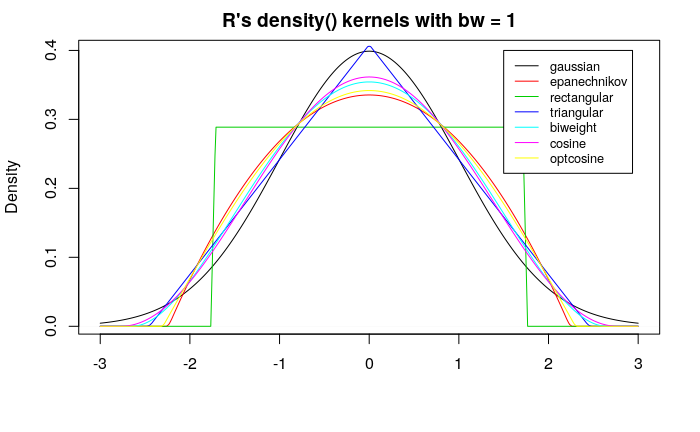
\includegraphics[width=0.8\textwidth]{figures/kernels.png}
    \caption{Kernels}
\end{figure*}
Then $\hat{f}\pa{b}$ where $\hat{f}$ is the N.W. estimator is biased. But a local polynomial estimator of order $\ge 1$ is consistent and unbiased.
\begin{remark}
    In TD, we will see that we can get a fast rate of convergence with nonnegative kernels (unlike in density estimation).
\end{remark}
\newpage


\end{document}
